\section{Induction Coupler Behaviors}

Of particular interest for the case of planar motion are induction couplers that include permanent magnets. Such an induction coupler consists of a mechanism that spins one or more permanent magnets at a variable speed. In its most elementary form, a permanent-magnet induction coupler uses only a single dipole that spins in a plane. However, each mechanism within the induction coupler can include any number of magnets. A large $\vert \textbf{B} \vert$ and $\nabla \textbf{B}$ maximizes the eddy-current force produced by the array of magnets. These properties can be achieved by using any number of dipoles orthogonal to the spin axis, or a circular Halbach array consisting of dipoles alternating between perpendicular and parallel to the spin axis.

\begin{figure}
\includegraphics[width = 6cm, height = 6cm ]{figures/Magnet_Arrays.png}

\caption{Different arrangement of permanent magnet arrays. Halbach array (left) and dipole array(right)}
\label{fig:magnet_arrays}
\end{figure}

The more magnets in an array, the more uniform the magnetic field becomes, smoothing the spatial variation in the magnetic field that the target sees. This smoothness decreases the change in the magnetic field as the magnets spin, which may be undesirable in an application that requires high eddy-current force. The number of magnets per array is one of the many considerations in the design of an induction coupler.

A straightforward example of an induction-coupler system is a single array spinning about an axis $\hat{\boldsymbol{a}}$ near conductive surface with a normal vector $\hat{\boldsymbol{n}}$. In this example, the force is 
\begin{equation}\label{eq:singlemagforce}
\textbf{F} = C\left[  \left(1-\beta \right )\hat{\boldsymbol{a}}{\times}\hat{\boldsymbol{n}} + \beta\hat{\boldsymbol{n}} \right ] \omega
\end{equation}

The factor $C$ scales spin speed of specific magnet arrays to the magnitude of the force they produce. $C$ is a function of the magnet properties, target properties, and $\boldsymbol{x}$. $\beta$ is the thrust ratio between the components of the force perpendicular and tangent to the target's surface. For small $\omega$, $\beta$ is small - see figure \ref{fig:tan_v_norm_f}, so the force is approximately tangential to the surface.

%%TODO CHANGE THIS FIGURE
\begin{figure}
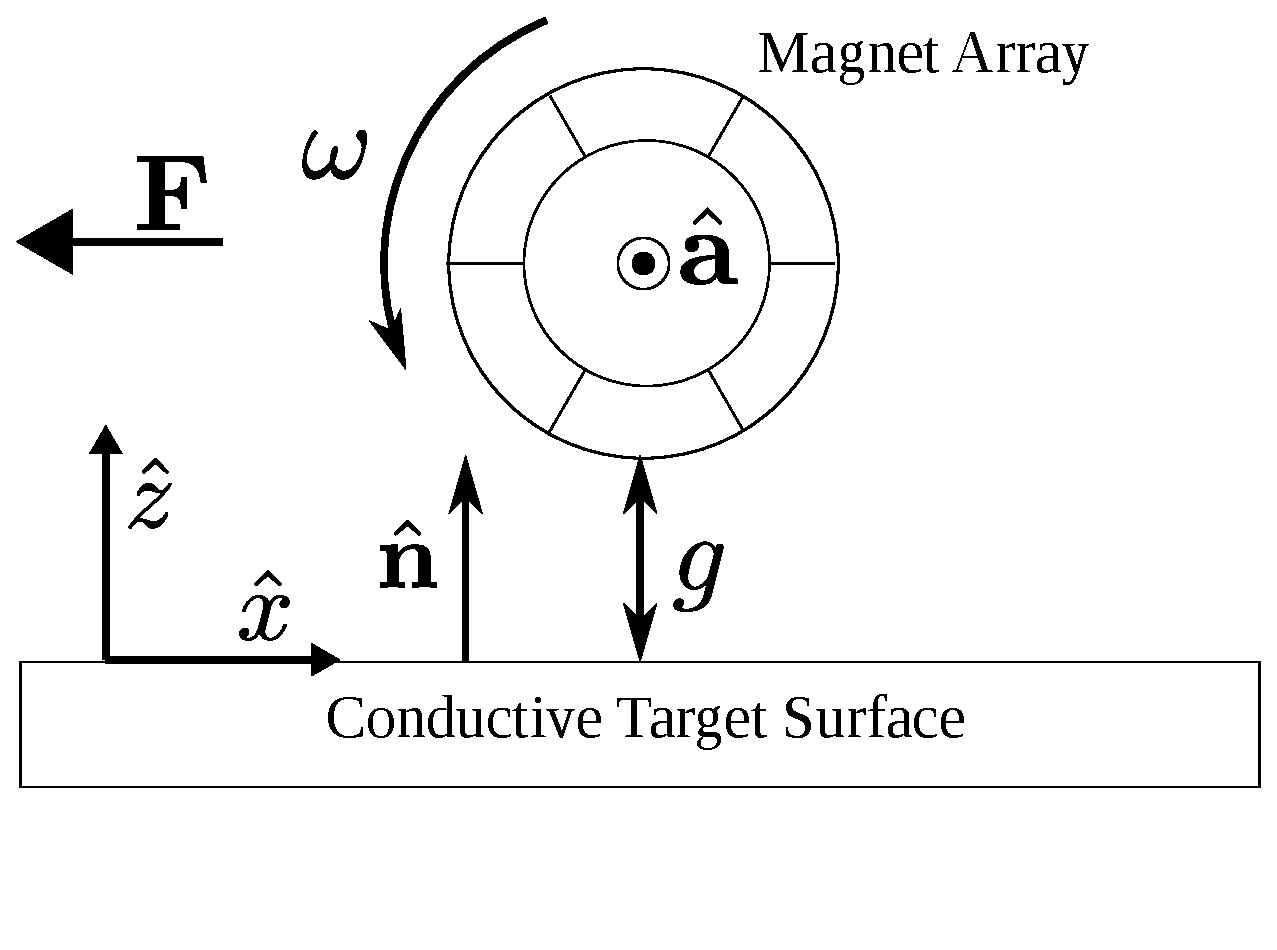
\includegraphics[width = 6cm, height = 6cm ]{figures/spin_mag_diagram.eps}

\caption{A dipole spinning with positive ($\omega$) about its axis $\hat{\textbf{a}}$ at distance g above a target that extends out of the page generates a force \textbf{F} directed to the left.}
\label{fig:arry_force_diagram}
\end{figure}

During in-plane movement, each array is associated with a single control degree of freedom. Its force and torque may project onto any of the six rigid-body degrees of freedom, depending upon geometries: the orientation of the coupler relative to the spacecraft's center of mass, distance between the coupler and the surface, and the topography of the surface. To first order, for a flat plate and a spin axis in a plane perpendicular to the surface normal, the effect is a force only, with no significant moment. The chaser spacecraft can use this force to torque itself if is the force acts at a moment arm relative to the chaser's center of mass. Alternatively, two couplers can create a moment through a couple, which is be independent of the coupler's position relative to the target's mass center.

%% BEN I THINK THIS FIGURE IS UNCESSARY
\begin{figure}
\includegraphics[width = 6cm, height = 6cm ]{figures/minimum_array.png}

\caption{A single-magnet induction coupler.}
\label{fig:min_array_diagram}
\end{figure}

\begin{figure}
\includegraphics[width = 6cm, height = 6cm ]{figures/tan_v_norm_force.png}

\caption{Shear and normal forces on the induction coupler under nominal operating conditions}
\label{fig:tan_v_norm_f}
\end{figure}

Experimental development of an induction coupler verifies models showing that this force varies with the magnitude and sign of $\omega$ and demonstrates that the couplers can produce milliNewton shear forces perpendicular to a surface for low power. Figure \ref{fig:force_plot} shows the input-output relationship between the motor speeds and the eddy-current forces they produce. In the demonstrations described here, force is achieved using two small COTS motors (BaneBots MP-36004-540) and neodymium magnets. Figure \ref{fig:cart_picture} shows the experiment  and table \ref{tab:exp_vals} shows the parameters used in the experiment.

\begin{table}
\caption{\label{tab:exp_vals} Experiment Values}
\begin{ruledtabular}
\begin{tabular}{ccc}
Variable & Value & Unit \\
\hline
 Motor Voltage & 12 & V\\
 Duty Cycle & 25 & \%max\\
 Motor Speed & 4200 & RPM \\
 Motor Current & 0.25 & A \\
 Motor Power & 0.75 & W \\
\end{tabular}
\end{ruledtabular}
\end{table}

\begin{table}
\caption{\label{tab:eforce_comparison} Specific Force Comparison}
\begin{ruledtabular}
\begin{tabular}{cc}
System & Specific Force (mN/W) \\
\hline
 Induction Couplers & 3.33 \\
 Electromagnetic Dipoles & 1.22 \cite{Kong2004} \\
 Coulomb Interactions & 3*$10^{-7}$ \cite{king2002spacecraft}\\
\end{tabular}
\end{ruledtabular}
\end{table}

\begin{figure}
\includegraphics[width = 6cm, height = 6cm ]{figures/cart_on_track.png}

\caption{An aluminum target on a low-friction air track (left) is moved by two spinning magnets (upper right.)}
\label{fig:cart_picture}
\end{figure}


\begin{figure}
\includegraphics[width = 6cm, height = 6cm ]{figures/motor_force_speed_plot.png}

\caption{Force on a one-dimensional air-track levitated cart vs. motor speed for a small, two-motor induction coupler. Oscillations in the force reported here are due to a combination of sensor artifacts and the dynamics of the cart.}
\label{fig:force_plot}
\end{figure}

The steady-state model of eddy-current forces makes two assumptions: that $\frac{1}{\omega}$ is much larger than the characteristic time of the LR circuit approximated by the bulk conductor and that the kinematics of the chaser and target are much slower than the period of rotation of the spinning magnetic fields that act on the target.

There are many other parameters governing induction-coupler force. The force magnitude decreases with $\frac{1}{g^4}$. Larger magnets provide stronger fields that increase the force. Greater thickness and 
conductivity of the target increase the induced current and thereby scale up the force. Spin speed increases the force nonlinearly by increasing the rate of change in the magnetic field. At low speeds this relationship is approximately linear (see fig. \ref{fig:lin_fit}) but increasing speed past a certain point shows diminishing returns because the penetration depth (or skin depth) of the induced current decreases at high frequencies. \cite{Paudel2013} The high dimensionality of this system motivates future work to algorithmically find suitable induction coupler design for different applications.